\documentclass[main_estudante.tex]{subfiles}

\begin{document}

\chapter{Transformações em gráficos}

\section{Questões diagnósticas}

\begin{diagnostico}
Esboce o gráfico de $p(x)=(x-1)(x+1)(x+3)$.
\end{diagnostico}

\section{Gabarito}

\textbf{Questão 1:} Os três detalhes importantes nessa representação gráfica são: as três raízes (-1, 1 e 3), o ponto em que o gráfico corta o eixo Y ($(0,3)$) e o comportamento do gráfico quando $x$ cresce positivamente (gráfico crescente) e quando $x$ cresce negativamente (gráfico decrescente).

\section{Quadro de orientação}

Neste capítulo, o quadro de orientação não é necessário, pois queremos que os estudantes passem por todas as questões. A questão diagnóstica desse ser usada apenas para lhe informar a respeito do ritmo que você deve esperar dos estudantes. Estudantes que tenham acertado a questão diagnóstica não devem ter dificuldade em esboçar gráficos e devem, portanto, avançar muito mais rapidamente ao longo das questões.

\section{Comentários iniciais}

Esse capítulo é inteiramente focado em gráficos. Seu objetivo mais explícito é trabalhar com as três transformações que podem ser realizadas em gráficos de funções através da soma e produto por uma constante. Esse conteúdo é abordado na seção 1.3 do livro \sugestao{Calculus}, ou seja, uma seção que já ficou para trás à bastante tempo. Nossa intenção é que a discussão feita aqui em tópicos que podem ser discutidos durante o Ensino Médio facilite o entendimento de aspectos que serão discutidos na disciplina de Cálculo em breve, quando derivadas forem usadas para auxiliar no esboo de gráficos.

Além disso, o capítulo tem a intenção indireta de reforçar uma habilidade mais básica que pode não ter sido dominada por muitos estudantes: o esboço de gráficos de funções.

Por conta do foco escolhido, esse capítulo tem um número menor de questões, mas espera-se que os estudantes gastem muito mais tempo nos itens que pedem o esboço de um gráfico. Dependendo do ritmo do seu grupo, pode ser que o capítulo não seja completado em dois encontros. Nesse caso, sugerimos que você \textbf{não} aloque mais encontros a ele pois acreditamos que a prática com o esboço de gráficos (mesmo que não tenha sido com todos os gráfico aqui propostos) já será benéfica aos estudantes.

\section{Questões comentadas}

\begin{questao}
Use os eixos cartesianos dados a seguir para  esboçar o gráfico das funções pedidas abaixo.
\begin{enumerate}[a)]
\item $f(x)=x+1$
\item $g(x)=x^2$
\item $h(x)=2^x$
\item $i(x)=sqrt{x}$
\item $j(x)=\sin(x)$
\item $l(x)=\cos(x)$
\end{enumerate}
\end{questao}

Essa primeira questão servirá de base para todo o capítulo. A ideia é que os estudantes obtenham novos gráficos e os comparem com esses. Portanto, é de fundamental importância que os gráficos aqui estejam bem feitos. Por essa razão sugerimos a lista de checagem logo após a questão e várias intruções antes dela. Insista para que ambas sejam seguidas, especialmente se seus estudantes falharam na questão diagnóstico.

\begin{questao}
Considerando os gráficos traçados anteriormente, faça o que se pede em cada item.
\begin{enumerate}[a)]
\item A função $f(x)$ é crescente ou decrescente?
\item Escreva os intervalos em que a função $g(x)$ é crescente e decrescente.
\item Identifique um trecho em que a função $l(x)=\cos(x)$ é crescente e outro em que ela é descrescente.
\end{enumerate}
\end{questao}

\begin{questao}
Considerando os gráficos traçados anteriormente, faça o que se pede em cada item.
\begin{enumerate}[a)]
\item Qual é a concavidade da função $g(x)$? Ela mantem essa mesma concavidade para todo o seu domínio?
\item Identifique um trecho em que a função $j(x)=\sin(x)$ tem concavidade positiva e outro com concavidade negativa.
\end{enumerate}
\end{questao}

O objetivo destas duas questões é introduzir um vocabulário que será muito utilizado em breve pelo professor de MA111. Como enfatizado no texto, não é importante se preocupar com o rigor dos conceitos mas com a interpretação visual deles. Use gestos e exemplos informais para explicar o significado de crescente/decrescente e de concavidade positiva ou negativa.

\begin{questao}
Usando como referência o gráfico de $h(x)$:
\begin{enumerate}[a)]
\item Esboce o gráfico das funções $a(x)=-(2^x)$ e $b(x)=2^{-x}$?
\item Como você descreveria o impacto causado pela multiplicação da função como um todo por $-1$ ($a(x)=-(2^x)$)?
\item Como você descreveria o impacto causado pela multiplicação da variável por $-1$ ($b(x)=2^{-x}$)?
\end{enumerate}
\end{questao}

\begin{questao}
Usando como referência o gráfico de $i(x)$:
\begin{enumerate}[a)]
\item Esboce o gráfico da função $c(x)=\sqrt(x)+2$.
\item Descreva o efeito gráfico de somarmos uma constante a uma função dada.
\item Descreva como seria o gráfico da função $c(x)=\sqrt(x)-1$.
\end{enumerate}
\end{questao}

Essas são as duas primeiras questões em que as funções iniciais são modificadas e o efeito nos seus gráficos são analisados. Incentive que os estudantes usem as suas palavras para descrever os efeitos, mas tente introduzir pouco a pouco termos mais precisos como reflexão em relação aos eixos e translação.

Se seus estudantes ainda precisarem da tabela de valores para esboçar os gráficos, dê tempo para que façam dessa forma. Essa prática é importante e mesmo que demorada deve promover habilidades importantes.

\begin{questao}
Usando como referência o gráfico de $l(x)$:
\begin{enumerate}[a)]
\item Esboce o gráfico da função $d(x)=2\cos(x)$.
\item Descreva o efeito gráfico de multiplicarmos uma função dada por uma constante.
\item O que ocorrerá se a constante for positiva, mas menor do que 1?
\item O que ocorrerá se a constante for negativa?
\end{enumerate}
\end{questao}

O efeito discutido nessa questão, informalmente tratado como um encolhimento ou esticamento pode ser descrito em termos da imagem da função ou, no caso de funções trigonométricas, de suas amplitudes. Aproveite a oportunidade para utilizar esses conceitos quando interagir com seus estudantes.

\begin{questao}
Usando como referência o gráfico de  $g(x)$:
\begin{enumerate}[a)]
\item Esboce os gráficos das funções $p(x)=x^2+1$ e $q(x)=(x+1)^2$.
\item Descreva o que aconteceu com o gráfico de $p(x)$.
\item Descreva o que aconteceu com o gráfico de $q(x)$.
\item Qual é a diferença do que foi feito com $g(x)$ para obter $p(x)$ e $q(x)$?
\item Qual transformação deve ser feita na função $e(x)=\sin(x)$ para que o seu gráfico se desloque horizontalmente 2 unidades para a direita?
\end{enumerate}
\end{questao}

Em funções periódicas, como as trigonométricas, o deslocamento horizontal é chamado de fase.

\begin{questao}
Usando como referência o gráfico de $e(x)$:
\begin{enumerate}[a)]
\item Esboce os gráficos das funções $t(x)=\sin(2x)$ e $u(x)=\sin(2\pi.x)$.
\item Qual é o período de cada uma das funções?
\item Como você descreveria o efeito na função seno de multiplicarmos a variável por uma constante?
\end{enumerate}
\end{questao}

O conceito de período é introduzido no enunciado dessa questão. Existe uma fórmula que costumava ser ensinada no Ensino Médio para resolver o item b, mas é importante que ela \textbf{não} seja usada nessa questão. Ao contrário, pode-se argumentar verbalmente algo como: a função seno completa seu ciclo quando $x$ varia de $0$ a $2\pi$ (pense no ciclo trigonométrico). Como $x$ está sendo multiplicado por $2$ (no caso da função $t(x)$), quando ele varia de $0$ até $\pi$, a multiplicação já varia de $0$ a $2\pi$, completando o ciclo ``antes''.

\begin{questao}
Usando a função $j(x)=\sin{x}$ como referência, obtenha a expressão algébrica de uma nova função satisfazendo cada uma das transformações abaixo.
\begin{enumerate}[a)]
\item Multiplicar a função por $2$.
\item Multiplicar a variável por $\frac{1}{4}$;
\item Somar $-1$ à função;
\item Somar $\pi$ à variável;
\end{enumerate}
\end{questao}

Nossa intenção não é de que os estudantes terminem este capítulo com uma lista de mudanças algébricas e seus efeitos no gráfico. O importante é que eles criem uma sensibilidade em relção a possíveis efeitos que mudanças simples podem causar no gráfico e, paralelamente, se sintam mais confortáveis em esboçar gráficos a partir de expressões algébricas acertando seus principais elementos. A intenção dessa questão é que os estudantes tenham alguma clareza sobre as diferentes mudanças que foram vistas ao longo do capítulo.

\begin{questao}
Esboce em um mesmo eixo cartesiano e \textbf{sem utilizar uma tabela de valores} o gráfico das quatro funções obtidas na questão anterior. Sugestão: use 4 cores diferentes.
\end{questao}

Como reforçado no enunciado, é importante que os estudantes tentem esboçar os gráficos sem utilizar tabelas de valores. Se eles não tiverem generalizado os efeitos discutidos, peça que voltem e encontrem as questões em que a mesma mudança algébrica tenha sido feita e analisam o efeito no gráfico.

\section{Rumo ao livro texto}

As questões discutida e resolvida deste capítulo lidam com o gráfico de funções sem que haja uma expressão algébrica estabelecida para elas. Trata-se de mais um passo de abstração dentro do conteúdo aqui discutido. Nenhuma dificuldade específica é esperada na questão proposta.

\section{Gabarito}

Confira as respostas para as questões e \textbf{não se esqueça de registrar o seu progresso}.

Questões sobre esboço de gráficos não terão gabarito, com exceção da questão 10.

\noindent\textbf{Questão 1:} Questão sem gabarito. Cheque a lista logo após a questão para cobrir características básicas de cada gráfico e pergunte a seu tutor se os esboços estão bons.

\noindent\textbf{Questão 2:} a) crescente, b) $g(x)$ é decrescente para $x<0$ e crescente para $x>0$.

\noindent\textbf{Questão 3:} a) concavidade positiva, b) no intervalo $0x<\pi$.

\noindent\textbf{Questão 4:} b) O gráfico foi refletido verticalmente, ou seja, em relação ao eixo $X$, c) O gráfico foi refletido horizontalmente, ou seja, em relação ao eixo $Y$.

\noindent\textbf{Questão 5:} b) o gráfico da função se desloca verticalmente, c) o gráfico se deslocaria para baixo, passando a assumirmos alguns valores positivos. Seu mínimo seria em $(0;-1)$ e raiz em $(1;0)$.

\noindent\textbf{Questão 6:} b) O gráfico da função é esticado verticalmente, b) O gráfico será encolhido verticalmente, c) O gráfico será refletido verticalmente e depois encolhido ou esticado, dependendo do módulo da constante.

\noindent\textbf{Questão 7:} b) Foi deslocado uma unidade para cima, c) Foi deslocado uma unidade para a esquerda, c) em $p(x)$ a constante foi soma à função e em $q(x)$ à variável, d) $e(x)=\sin(x-2)$.

\noindent\textbf{Questão 8:} b) O periodo de $t(x)$ é $\pi$ e o de $u(x)$ é $1$, c) O gráfico da função é encolhido horizontalmente. Se a função for periódica, podemos dizer que o seu período foi alterado.

\noindent\textbf{Questão 9:} a) $j_a(x)=2\sin(x)$, b) $j_b(x)=\sin(x/4)$, c)$j_c(x)=\sin(x)-1$, $j_d(x)=\sin(x+\pi)$.

\noindent\textbf{Questão 10:}

\begin{figure}[h]
\centering
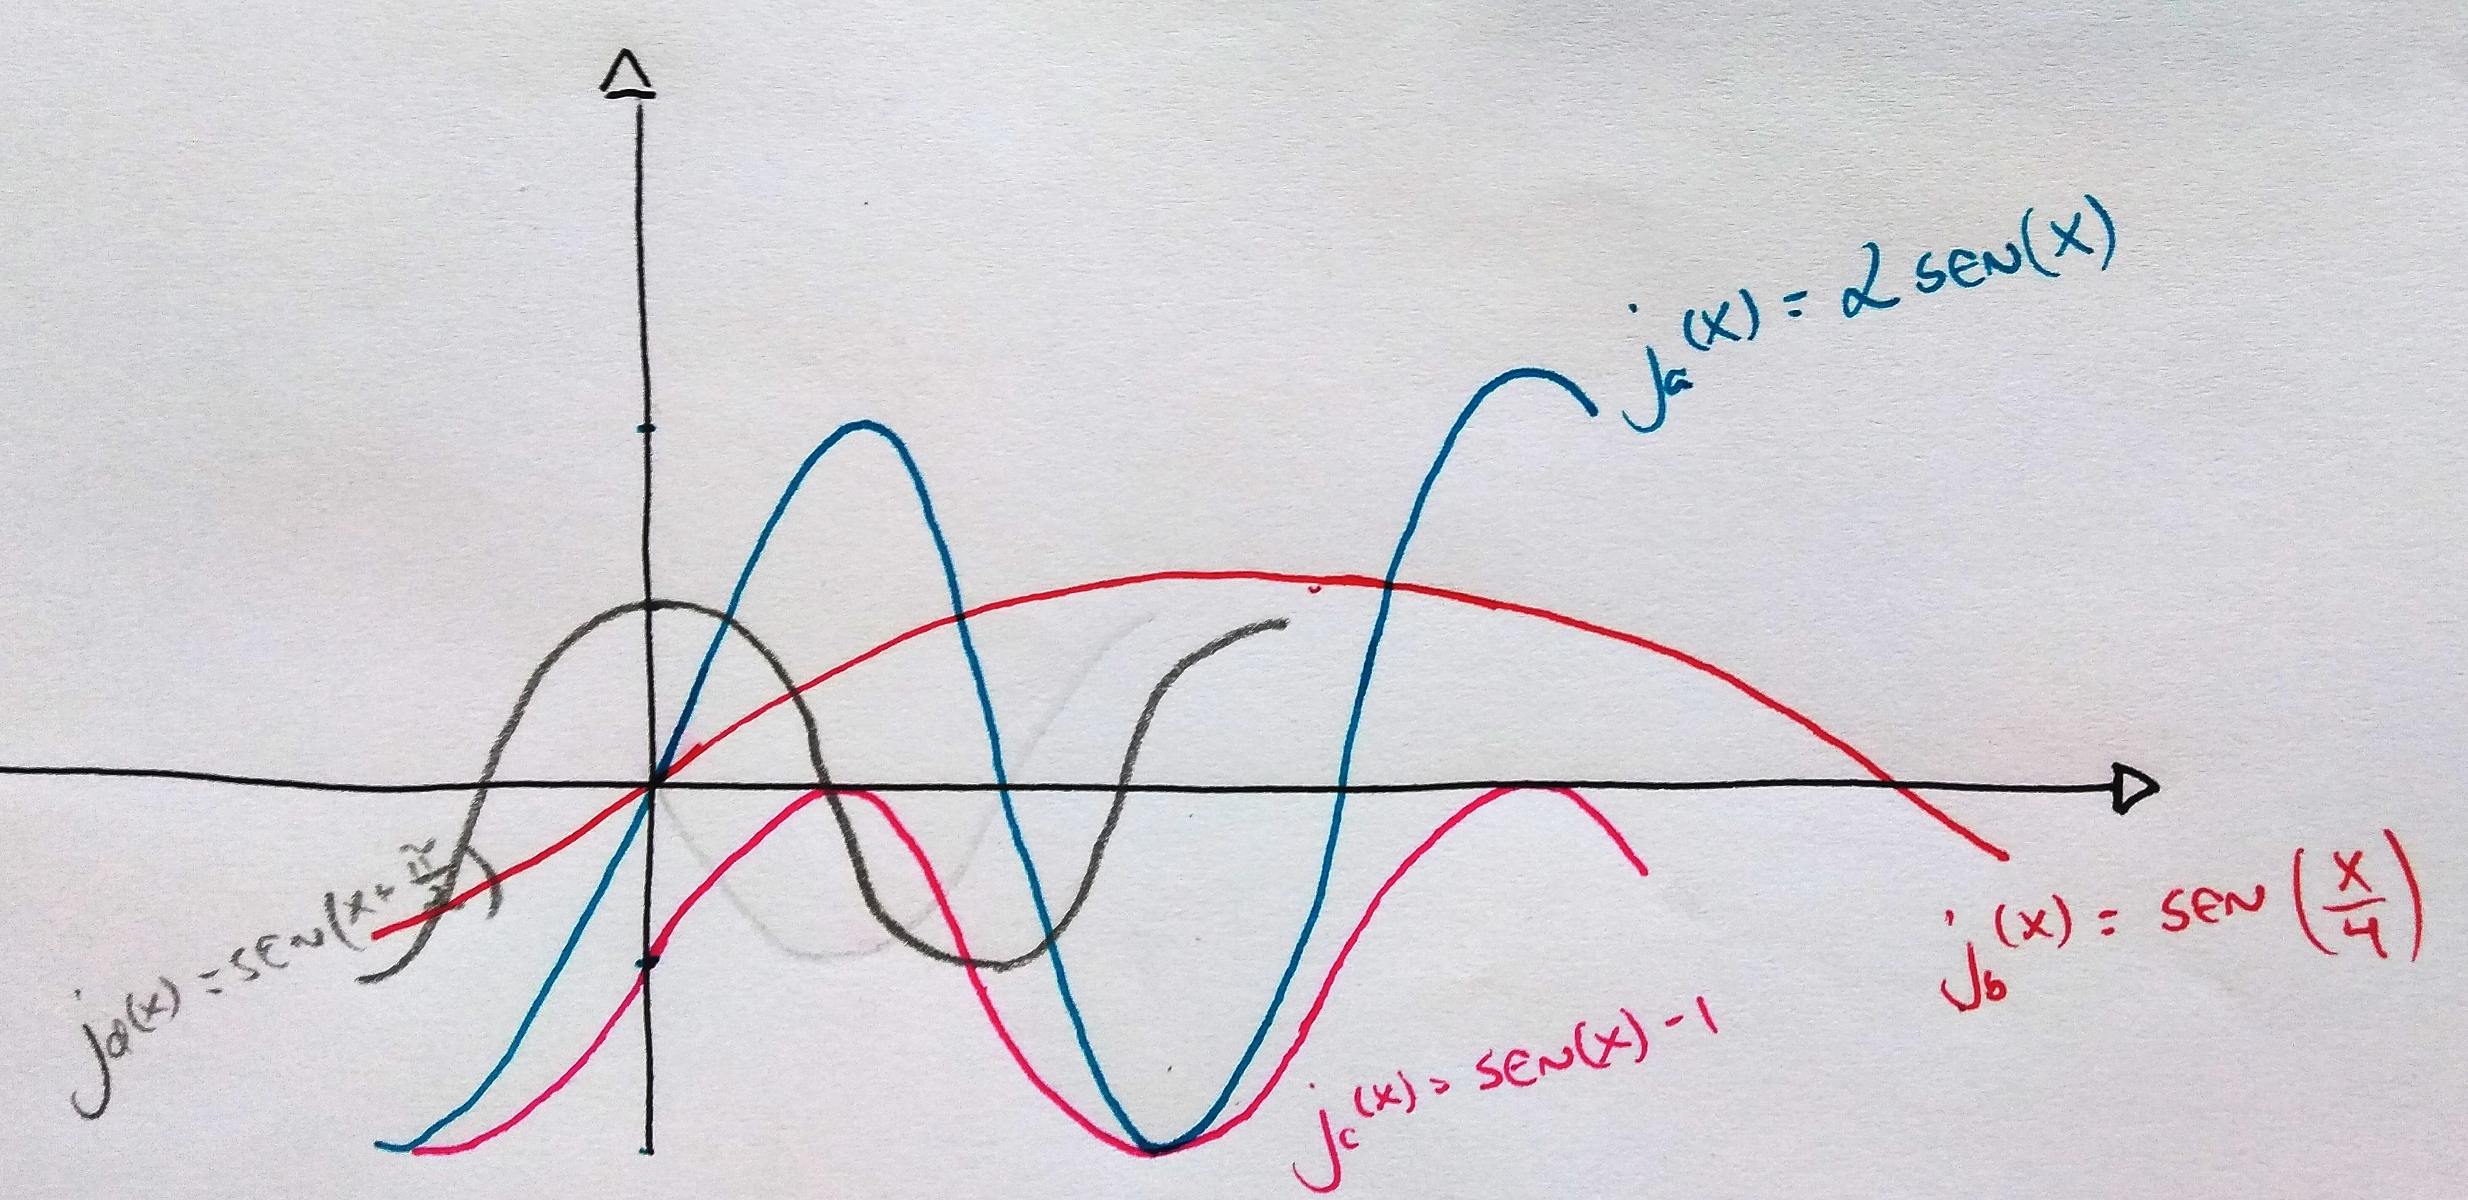
\includegraphics[width=0.75\textwidth]{./img/c7g10.jpg}
\end{figure}

\section{Questões adicionais}

Ao longo do capítulo não foram sugeridas questões que pedem a expressão algébrica a partir de características gráficas de funções. Esse tipo de questão pode ser útil para gerar questões adicionais como a seguinte.

\begin{questao}
Obtenha a expressão algébrica para funções dentro das restrições gráficas descritas em cada item.
\begin{enumerate}[a)]
\item Obtenha uma função seno cujo período seja igual a $1$ e a imagem seja igual ao intervalo $1 \leq y \leq 3$.
\item Obtenha uma função quadrática cujo vértice esteja no ponto $(2,-1)$.
\end{enumerate}
\end{questao}

Você pode gerar variações em torno dessa questões, especialmente usando as funções trigonométricas. No geral, acrescentar a fase (a constante somadaà variável) dificulta bastante a questão.

A seção 3.8 do livro \sugestao{MAtemática básica - volume 1} é muito compatível com o conteúdo deste capítulo. Você pode sugerir uma leitura deste material ou exercícios propostos na lista ao final dele. A única diferença é que a função módulo também é utilizada pelo autor.

\end{document}
